\documentclass[final, 3p, times, 11.5pt]{article}

\usepackage[english]{babel}
\usepackage[utf8]{inputenc}
\usepackage[T1]{fontenc}

% Dokumentformatering:
\setlength\parindent{0pt} %ingen innrykk
\usepackage[parfill]{parskip} % Mellomrom mellom avsnitt
% Endre str
\usepackage[a4paper,top=3cm,bottom=2cm,left=1.5cm,right=1.5cm,marginparwidth=1.75cm]{geometry} % utnytter større del av arket.
\usepackage{appendix}
\usepackage{multicol}
\usepackage{titlesec}
\titleformat{\chapter}[display]
  {\normalfont\huge\bfseries}{\chaptertitlename\ \thechapter}{20pt}{\Huge}
\titlespacing*{\chapter}{0pt}{-70pt}{20pt} % reduce headspace of the chapter title
\setcounter{secnumdepth}{0} % Set the depth of section numbering to subsubsections



% Matte og symboler
\usepackage{lmodern}
\usepackage{textcomp, gensymb}
\usepackage{amssymb}
\usepackage{amsmath}
\usepackage{mathtools}
\usepackage{physics}
\usepackage{cancel} % Gjennomstreking i likninger etc
\usepackage{amsthm}
\usepackage{caption}
\usepackage{dirtytalk}
\usepackage{cancel}

% Pseudocode
\usepackage{algorithm}
\usepackage{algpseudocode}

% Håndterer grafikk:
\usepackage{graphicx}
\graphicspath{{Figures/}} % Henter grafikk fra mappen "Figurer"
\usepackage{wrapfig}
\setlength{\intextsep}{2pt} % adjust vertical space above and below the wrapfigure
\usepackage{subcaption} % eller subfigure
\usepackage[font=small,labelfont=bf]{caption} % Mindre figurtekst, bold på figur numerering
\usepackage{transparent} % Kan gjøre tekst mere gjenomsiktig
\usepackage{listings}
\usepackage{paralist}
\usepackage{tikz}
\usetikzlibrary{matrix}
\usetikzlibrary{fit}
\usetikzlibrary{intersections}
\usepackage{multirow}
\usepackage{pdfpages} % sett in pdf i dokumentet
\usepackage{subcaption} 
\usepackage{tabularx}
\usepackage{tabularray} % beste tabellpakke
\usepackage{pgfplots}
\usepgfplotslibrary{fillbetween}
\pgfplotsset{width=10cm,compat=1.9}
\newcommand{\tabitem}{~~\llap{\textbullet}~~} % for kulepunkter i tabeller uten vspace over dem

% Håndterer fine tabeller:
\usepackage{booktabs}
\usepackage{multirow}

% Håntere kilder med hyperlinker
\usepackage{csquotes}
\usepackage{hyperref}
\hypersetup{
    colorlinks=true,        % Colored links instead of frames
    linkcolor=blue,         % Color for internal links
    citecolor=red,          % Color for citations
    urlcolor=red            % Color for external links
}
\usepackage[style=numeric, sorting=none]{biblatex} 
\addbibresource{sources.bib}
\usepackage{lastpage} 
\usepackage[printonlyused,withpage]{acronym}
\usepackage{footmisc}




% Egne funksjoner
\newcommand{\frontmatter}{\cleardoublepage \pagenumbering{roman}}
\newcommand{\mainmatter}{\cleardoublepage \pagenumbering{arabic}}

\usepackage{caption}
\captionsetup{%
    ,format=hang
    ,justification=raggedright
    ,singlelinecheck=false
    ,figureposition=top
    }


\makeatletter
\AtBeginDocument{%
  \renewcommand*{\AC@hyperlink}[2]{%
    \begingroup
      \hypersetup{hidelinks}%
      \hyperlink{#1}{#2}%
    \endgroup
  }%
}
\makeatother





% Håndterer multi-fil oppsett:
\usepackage{xr}
\usepackage{subfiles}
\externaldocument{\subfix{main}}
 

\begin{document}
\section{Problem 5}

To test the effect of increasing the democratization resolution (that is, letting $n$ grow), we simply iterate over different sizes in $\mathbf{N} = \{2, 4, 8, 16, 32, 64, 128\}$. 

As shown in table \ref{tab:conv} number of iterations used for convergence of the algorithm increases exponentially with an increase in the discretization resolution. The fractional relation between iterations and $N$ is computed in the last column.

\begin{table}[h!]
    \centering
    \caption{Relationship between discretization resolution $n$ (represented by $N = n-1$),  and how many iterations that were performed. }
    \begin{tabular}{llll}
    \hline
    N & Iterations & Ierations / N \\ \hline \hline
2.0 & 1.0 & 0.500000 \\
4.0 & 6.0 & 1.500000 \\
8.0 & 81.0 & 10.125000 \\
16.0 & 376.0 & 23.500000 \\
32.0 & 1541.0 & 48.156250 \\
64.0 & 6413.0 & 100.203125 \\
128.0 & 25823.0 & 201.742188 \\
256.0 & 104206.0 & 407.054688 \\
512.0 & 419619.0 & 819.568359 \\ \hline
    \end{tabular}
    \label{tab:conv}
\end{table}

In the LHS plot of figure \ref{fig:p2prob5} we see the iterations for convergence as a function of $N$. The \say{Type} legend indicates:
\begin{itemize}
    \item \textbf{Tridiagonal} - is the same matrix as in table \ref{tab:conv} as presented in problem 2.
    \item \textbf{Tridiagonal w.o 1/h\^ 2} - We have factored out 1/h\^ 2 from A thus altering the order from $\mathcal{O}(10)$ to $\mathcal{O}(1)$.
    \item \textbf{Random symmetric} - is a matrix where the elements are filled in randomly with numbers from the gaussian distribution $\sim N(0, 1)$ and then we make it symmetric by mirroring the upper triangle onto the lower. Here all cells will be non-zero. but their order of magnitude will be small.
\end{itemize}

These results indicates how both the order of magnitude and number of non zero off-diagonal elements affects the number of iterations. In ht RHS plot we see that the crowth rate of the relation Iterations/N is approximately linear as a function of $N$ and resides somewhere between the 1to 1 and 2 to 1 line for the three different matrice types.
\begin{figure}[h!]
    \centering
    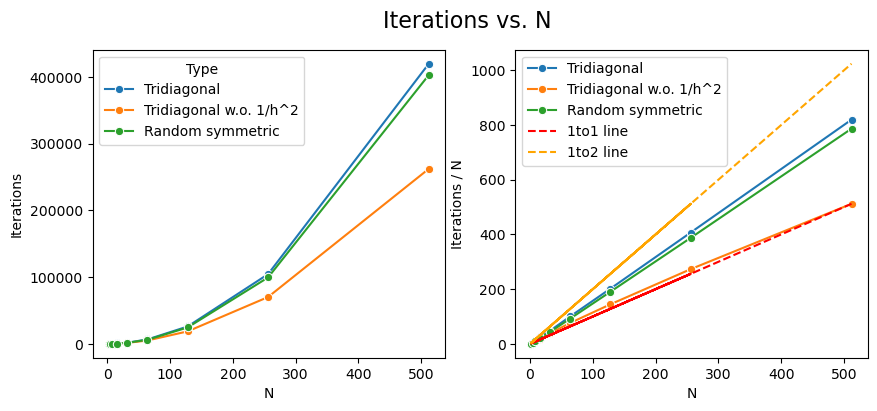
\includegraphics[width=0.7\linewidth]{Project 2/Figures/output.png}
    \caption{LHS: the iterations for convergence as a function of $N$. \\
    RHS: iterations/N as a function of $N$.}
    \label{fig:p2prob5}
\end{figure}


\end{document}


